\chapter{Analisis Keamanan}
\label{ch:analisis}

Bab ini membahas hasil pengujian \textit{avalanche effect}, entropi, dan histogram, lalu dilanjutkan dengan pengujian tambahan terhadap komponen rancangan. Pengujian tingkat blok dijalankan dengan \code{test/test\_security.py}, yang keluaran lengkapnya terdapat pada \cref{app:security}. Pengujian tingkat berkas memakai berkas dan kunci yang sama dengan \cref{ch:implementasi}.

\section{Avalanche Effect}

\subsection{Tingkat Blok}
Uji \textit{avalanche} paling bersih dilakukan pada satu blok dengan \textit{round key} tetap, agar pengaruh \textit{nonce} acak tidak ikut terhitung. Untuk 20 blok acak, setiap bit dari 256 bit \textit{plaintext} dibalik satu per satu (total 5.120 pasangan), lalu dihitung jarak Hamming antara kedua \textit{ciphertext}. Hal yang sama dilakukan untuk setiap bit kunci ke-4 (64 pasangan) dengan \textit{nonce} tetap. Hasilnya ditunjukkan pada \cref{tab:avalanche-blok}.

\begin{table}[H]
    \centering
    \caption{\textit{Avalanche effect} tingkat blok (256 bit)}
    \label{tab:avalanche-blok}
    \begin{tabular}{l r r r}
        \toprule
        \textbf{Perubahan 1 bit pada} & \textbf{Rata-rata} & \textbf{Minimum} & \textbf{Maksimum} \\
        \midrule
        \textit{Plaintext} & 49,95\% & 98 bit (38,3\%) & 162 bit (63,3\%) \\
        Kunci & 50,46\% & 115 bit (44,9\%) & -- \\
        \bottomrule
    \end{tabular}
\end{table}

Rata-rata keduanya sangat dekat dengan nilai ideal 50\%. Rentang 98--162 bit juga konsisten dengan distribusi binomial $\mathrm{B}(256, \tfrac12)$, yang memiliki simpangan baku 8 bit. Nilai ekstrem 98 dan 162 bit berjarak sekitar 3,8 dan 4,3 simpangan baku dari rata-rata 128. Dengan 5.120 sampel, peluang munculnya minimal satu nilai sejauh 4,3 simpangan baku secara kebetulan sekitar 10\%, sehingga hasil ini sesuai dengan perilaku permutasi acak.

\subsection{Difusi terhadap Jumlah Ronde}
Untuk melihat seberapa cepat difusi tercapai, \textit{avalanche} diukur ulang dengan hanya menjalankan $n$ ronde pertama, untuk $n = 1, \dots, 18$ (\cref{fig:difusi}). Difusi penuh (sekitar 50\%) tercapai setelah \textbf{4 ronde}. Hal ini sesuai dengan struktur Feistel: satu bit di $R_0$ memengaruhi seluruh $R_1$ melalui $F$, lalu membutuhkan satu ronde lagi untuk menyebar ke paruh lainnya. Dengan 18 ronde, \algname{} memiliki margin keamanan sekitar 4,5 kali jumlah ronde minimum untuk difusi penuh. Margin ini sebanding dengan AES-128, yang mencapai difusi penuh setelah 2 ronde dan memakai 10 ronde.

\begin{figure}[H]
    \centering
    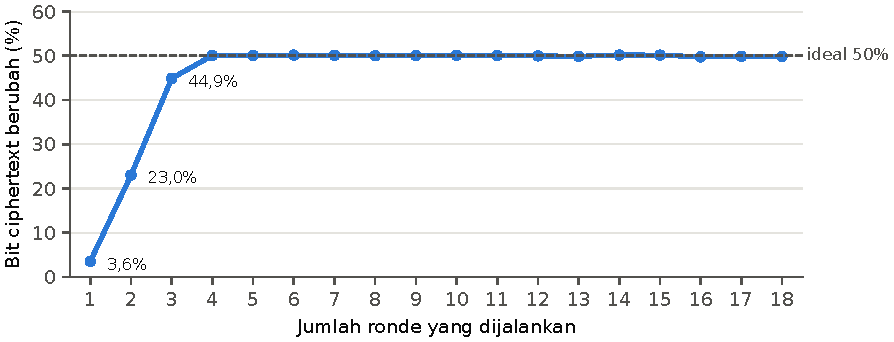
\includegraphics[width=\textwidth]{diffusion_rounds.pdf}
    \caption{Persentase bit \textit{ciphertext} yang berubah terhadap jumlah ronde yang dijalankan (12 blok $\times$ 64 posisi bit per titik)}
    \label{fig:difusi}
\end{figure}

\subsection{Tingkat Berkas pada Setiap Mode}
\Cref{tab:avalanche-mode} menunjukkan \textit{avalanche} pada 2.048 byte pertama setiap berkas (seluruh isi untuk \code{glasses.txt}). \textit{Nonce} yang sama dipakai untuk kedua enkripsi, dan bit yang dibalik adalah bit pertama \textit{plaintext} atau bit terakhir byte pertama kunci.

\begin{table}[H]
    \centering
    \caption{\textit{Avalanche effect} tingkat berkas per mode operasi}
    \label{tab:avalanche-mode}
    \begin{tabular}{l r r r r}
        \toprule
        \multirow{2}{*}{\textbf{Mode}} & \multicolumn{2}{c}{\textbf{1 bit \textit{plaintext}}} & \multicolumn{2}{c}{\textbf{1 bit kunci}} \\
        \cmidrule(lr){2-3} \cmidrule(lr){4-5}
        & \code{glasses.txt} & \code{image.jpg} & \code{glasses.txt} & \code{image.jpg} \\
        \midrule
        ECB & 1,46\% & 0,72\% & 50,27\% & 50,67\% \\
        CBC & 49,89\% & 49,87\% & 49,47\% & 50,52\% \\
        CFB & 48,88\% & 49,18\% & 50,39\% & 50,57\% \\
        OFB & 0,01\% & 0,01\% & 50,66\% & 50,79\% \\
        CTR & 0,01\% & 0,01\% & 50,79\% & 49,95\% \\
        \bottomrule
    \end{tabular}
\end{table}

Perubahan \textbf{kunci} menghasilkan \textit{avalanche} sekitar 50\% pada kelima mode, karena seluruh \textit{round key} ikut berubah. Sebaliknya, \textit{avalanche} terhadap perubahan \textbf{\textit{plaintext}} sangat bergantung pada mode:
\begin{itemize}
    \item \textbf{CBC dan CFB} (sekitar 50\%): perubahan pada blok pertama merambat ke semua blok berikutnya melalui rantai umpan balik.
    \item \textbf{ECB} (1,46\% dan 0,72\%): hanya blok pertama yang berubah, dan sekitar setengah bitnya berubah. Karena blok pertama hanya 1/33 dan 1/65 bagian dari data yang diukur (termasuk blok \textit{padding}), persentase totalnya kecil.
    \item \textbf{OFB dan CTR} (0,01\% = tepat 1 bit): aliran kunci tidak bergantung pada \textit{plaintext}, sehingga membalik satu bit \textit{plaintext} hanya membalik satu bit yang sama di \textit{ciphertext}.
\end{itemize}
Nilai kecil pada ECB, OFB, dan CTR \textbf{bukan kelemahan \textit{block cipher}}, melainkan sifat bawaan mode tersebut yang juga berlaku pada AES. Hasil tingkat blok pada \cref{tab:avalanche-blok} menunjukkan bahwa fungsi $E$ sendiri memiliki \textit{avalanche} yang ideal. Hal ini juga menjelaskan mengapa \code{src/analysis.py} memakai mode CBC untuk pengukuran \textit{avalanche}.

\section{Entropi}
Entropi Shannon dihitung pada \textit{ciphertext} mentah tanpa \textit{nonce}. Base64 tidak dipakai karena hanya memiliki 64 simbol, sehingga entropinya tidak mungkin melebihi 6 bit per byte. Hasilnya ditunjukkan pada \cref{tab:entropi}.

\begin{table}[H]
    \centering
    \caption{Entropi Shannon (bit per byte, maksimum 8) \textit{plaintext} dan \textit{ciphertext}}
    \label{tab:entropi}
    \begin{tabular}{l r r r r r r r}
        \toprule
        \multirow{2}{*}{\textbf{Berkas}} & \multirow{2}{*}{\textbf{\textit{Plaintext}}} & \multicolumn{5}{c}{\textbf{\textit{Ciphertext}}} & \multirow{2}{*}{\textbf{Harapan acak}} \\
        \cmidrule(lr){3-7}
        & & ECB & CBC & CFB & OFB & CTR & \\
        \midrule
        \code{glasses.txt} & 4,3935 & 7,7762 & 7,8292 & 7,8137 & 7,8386 & 7,8077 & 7,8258 \\
        \code{image.jpg}   & 7,9306 & 7,9997 & 7,9998 & 7,9998 & 7,9998 & 7,9998 & 7,9998 \\
        \code{video.mp4}   & 7,9993 & -- & 8,0000 & -- & -- & -- & 8,0000 \\
        64 KB byte nol     & 0,0000 & -- & 7,9973 & -- & -- & -- & 7,9972 \\
        \bottomrule
    \end{tabular}
\end{table}

Entropi \textit{ciphertext} \code{glasses.txt} (7,78--7,84) tampak lebih rendah daripada berkas lain, tetapi nilai ini memang yang diharapkan dari data acak sempurna berukuran sama. Entropi yang diukur dari sampel berhingga sebanyak $n$ byte bersifat bias ke bawah, dengan nilai harapan sekitar \cite{miller1955}
\begin{equation}
    \mathbb{E}[\hat{H}] \approx 8 - \frac{255}{2n \ln 2}.
\end{equation}
Untuk $n = 1.056$ byte, nilai harapannya 7,8258, sehingga hasil 7,78--7,84 sesuai dengan keluaran yang acak. Untuk citra ($n = 833.312$), nilai harapannya 7,9998, dan untuk video ($n = 39.228.672$) nilai harapannya 7,999995. Keduanya sama dengan hasil pengukuran. Video MP4 yang sudah terkompresi memiliki entropi \textit{plaintext} 7,9993, sehingga entropi saja tidak dapat membedakan \textit{plaintext} terkompresi dari \textit{ciphertext}. Karena itu, histogram dan uji $\chi^2$ pada subbab berikutnya tetap diperlukan. Kasus paling ekstrem adalah 64 KB byte nol (entropi \textit{plaintext} 0): \textit{ciphertext}-nya tetap mencapai entropi 7,9973. Artinya, keacakan keluaran tidak bergantung pada keacakan masukan.

\section{Histogram}
\Cref{fig:hist-teks,fig:hist-citra,fig:hist-video} membandingkan histogram nilai byte \textit{plaintext} dan \textit{ciphertext} (mode CBC). Histogram \textit{plaintext} teks terkonsentrasi pada rentang huruf ASCII (sekitar 97--122) dan spasi (32). Histogram citra JPEG tidak rata, dengan puncak paling menonjol di nilai \code{0x00} (sekitar 2,7 kali rata-rata). Setelah dienkripsi, kedua histogram menjadi rata di sekitar nilai harapan (garis putus-putus), tanpa sisa pola dari \textit{plaintext}.

\begin{figure}[H]
    \centering
    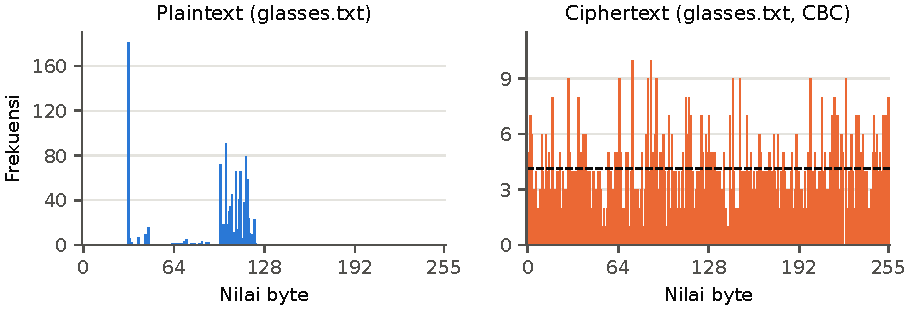
\includegraphics[width=\textwidth]{hist_text.pdf}
    \caption{Histogram \code{glasses.txt}: \textit{plaintext} (kiri) dan \textit{ciphertext} CBC (kanan). Garis putus-putus menunjukkan frekuensi harapan distribusi seragam.}
    \label{fig:hist-teks}
\end{figure}

\begin{figure}[H]
    \centering
    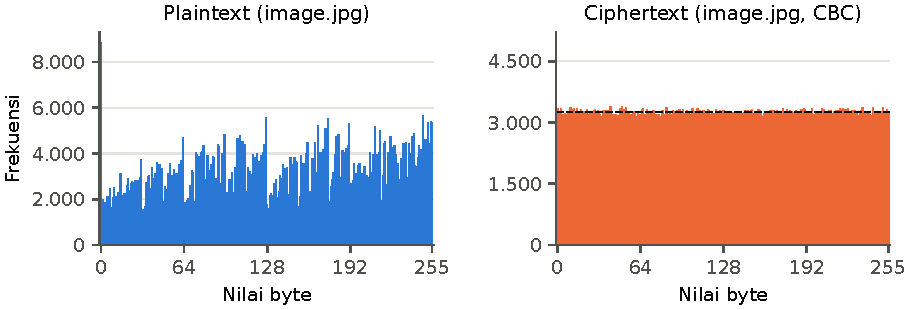
\includegraphics[width=\textwidth]{hist_image.pdf}
    \caption{Histogram \code{image.jpg}: \textit{plaintext} (kiri) dan \textit{ciphertext} CBC (kanan)}
    \label{fig:hist-citra}
\end{figure}

\begin{figure}[H]
    \centering
    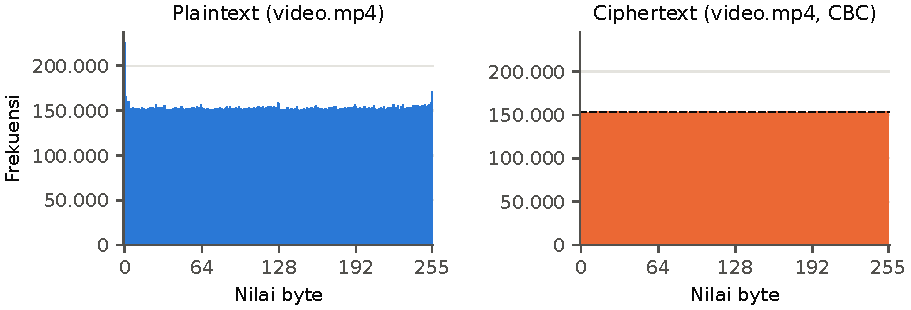
\includegraphics[width=\textwidth]{hist_video.pdf}
    \caption{Histogram \code{video.mp4}: \textit{plaintext} (kiri) dan \textit{ciphertext} CBC (kanan)}
    \label{fig:hist-video}
\end{figure}

Kerataan histogram diuji secara kuantitatif dengan uji $\chi^2$ (255 derajat kebebasan, nilai kritis 293,25 pada $\alpha = 5\%$). Hasilnya ditunjukkan pada \cref{tab:chi2}.

\begin{table}[H]
    \centering
    \caption{Statistik $\chi^2$ histogram (lolos jika $< 293{,}25$)}
    \label{tab:chi2}
    \begin{tabular}{l r r r r r r}
        \toprule
        \textbf{Berkas} & \textbf{\textit{Plaintext}} & \textbf{ECB} & \textbf{CBC} & \textbf{CFB} & \textbf{OFB} & \textbf{CTR} \\
        \midrule
        \code{glasses.txt} & 17.551 & 309,3$^{*}$ & 241,5 & 257,0 & 224,5 & 264,2 \\
        \code{image.jpg}   & 81.473 & 304,1$^{*}$ & 228,4 & 250,7 & 262,4 & 252,9 \\
        \code{video.mp4}   & 42.092 & -- & 252,4 & -- & -- & -- \\
        64 KB byte nol     & -- & -- & 239,6 & -- & -- & -- \\
        \bottomrule
    \end{tabular}
\end{table}

Seluruh \textit{ciphertext} pada mode CBC, CFB, OFB, dan CTR, serta \textit{ciphertext} video dan berkas nol, lolos uji $\chi^2$. Dua nilai pada mode ECB melewati batas: 309,3 pada berkas teks ($p \approx 0{,}011$) dan 304,1 pada citra ($p \approx 0{,}019$). ECB memang memetakan blok \textit{plaintext} identik ke blok \textit{ciphertext} identik, sehingga kami terlebih dahulu memeriksa apakah blok berulang menjadi penyebabnya. Ternyata \code{glasses.txt} tidak memiliki blok 32 byte yang berulang, dan \code{image.jpg} hanya memiliki 33 blok duplikat dari 26.040 blok, jumlah yang terlalu kecil untuk memengaruhi histogram. Karena itu, kami mengulang enkripsi berkas teks sebanyak 300 kali dengan \textit{nonce} berbeda untuk setiap mode, dan mengulang enkripsi ECB citra sebanyak 20 kali (\cref{tab:chi2-ulang}).

\begin{table}[H]
    \centering
    \caption{Distribusi $\chi^2$ dari enkripsi ulang dengan \textit{nonce} berbeda}
    \label{tab:chi2-ulang}
    \begin{tabular}{l r r r r}
        \toprule
        \textbf{Mode} & \textbf{Rata-rata} & \textbf{Simpangan baku} & \textbf{Melewati 293,25} & \textbf{Maksimum} \\
        \midrule
        \multicolumn{5}{l}{\textit{\code{glasses.txt}, 300 kali per mode}} \\
        ECB & 255,8 & 22,8 & 7,0\% & 314,7 \\
        CBC & 254,6 & 21,9 & 3,7\% & 331,6 \\
        CFB & 255,1 & 21,5 & 5,3\% & 333,1 \\
        OFB & 256,2 & 23,0 & 6,0\% & 323,4 \\
        CTR & 255,1 & 21,4 & 3,0\% & 341,8 \\
        \midrule
        \multicolumn{5}{l}{\textit{\code{image.jpg}, 20 kali}} \\
        ECB & 253,8 & 24,8 & 15\% (3 dari 20) & 300,7 \\
        \midrule
        Teoretis $\chi^2_{255}$ & 255,0 & 22,6 & 5,0\% & -- \\
        \bottomrule
    \end{tabular}
\end{table}

Pada kelima mode, rata-rata dan simpangan baku $\chi^2$ sesuai dengan distribusi teoretis $\chi^2_{255}$. Proporsi yang melewati batas (3,0--7,0\%) berada dalam sekitar 1,6 galat baku dari nilai nominal 5\% (galat baku $\pm 1{,}3\%$ untuk 300 percobaan). Pada citra, 3 dari 20 percobaan ECB melewati batas, tetapi peluang mendapatkan minimal 3 kegagalan dari 20 percobaan secara kebetulan sekitar 7,5\%, dan rata-ratanya (253,8) tetap sesuai harapan. Enkripsi CTR atas 1 MB byte nol juga menghasilkan $\chi^2 = 238{,}8$. Dengan demikian, kegagalan pada \cref{tab:chi2} merupakan fluktuasi acak, bukan bias pada mode tertentu.

\section{Pengujian Tambahan}

\subsection{Kebocoran Pola pada Mode ECB}
Kelemahan klasik ECB diuji dengan citra mentah berukuran $256 \times 256$ piksel \textit{grayscale} (1 byte per piksel) yang memiliki banyak area seragam (\cref{fig:ecb}). Citra ini memiliki 2.048 blok, tetapi hanya 270 blok yang berbeda. Pada ECB, \textit{ciphertext}-nya juga memiliki tepat 270 blok berbeda, sehingga bentuk-bentuk pada citra masih terlihat jelas. Pada CBC dan CTR, ke-2.048 blok \textit{ciphertext} semuanya berbeda dan citra tampak seperti derau. Percobaan dengan 100 blok \textit{plaintext} identik menunjukkan hal yang sama: ECB hanya menghasilkan 2 blok \textit{ciphertext} berbeda, yaitu blok data dan blok \textit{padding}.

\begin{figure}[H]
    \centering
    \begin{subfigure}{0.23\textwidth}\centering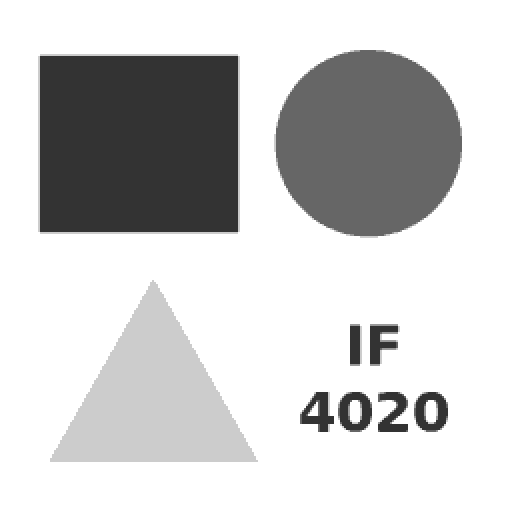
\includegraphics[width=\linewidth]{ecb_plain.png}\caption{\textit{Plaintext}}\end{subfigure}\hfill
    \begin{subfigure}{0.23\textwidth}\centering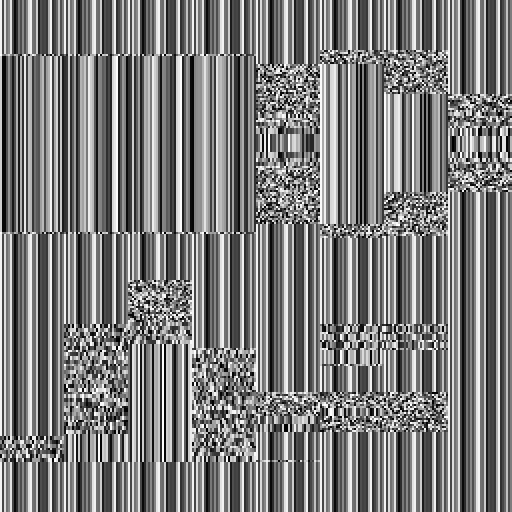
\includegraphics[width=\linewidth]{ecb_ecb.png}\caption{ECB}\end{subfigure}\hfill
    \begin{subfigure}{0.23\textwidth}\centering
\includegraphics[width=\linewidth]{ecb_cbc.png}\caption{CBC}\end{subfigure}\hfill
    \begin{subfigure}{0.23\textwidth}\centering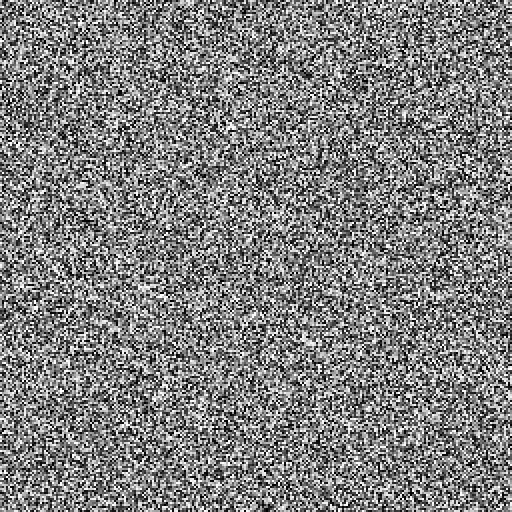
\includegraphics[width=\linewidth]{ecb_ctr.png}\caption{CTR}\end{subfigure}
    \caption{Citra mentah yang dienkripsi dengan ECB, CBC, dan CTR (setiap baris citra 256 piksel = 8 blok)}
    \label{fig:ecb}
\end{figure}

\textit{Nonce} per pesan membuat \algname{} lebih baik daripada ECB pada AES dalam satu hal: blok yang sama pada \textbf{dua pesan berbeda} menghasilkan \textit{ciphertext} berbeda, karena \textit{round key}-nya berbeda. Namun, di \textbf{dalam satu pesan}, ECB tetap membocorkan pola, sehingga mode ini tidak disarankan untuk data berpola.

\subsection{Analisis Kotak-S dan Iterasi Desain}
\label{sec:iterasi-sbox}
Versi awal $f_{\text{SPN}}$ memakai Kotak-S afin $S(x) = (167x + 91) \bmod 256$. Analisis diferensial menunjukkan bahwa selisih $\Delta = \texttt{0x80}$ pada setiap byte lolos melalui seluruh komponen $f_{\text{SPN}}$:
\begin{itemize}
    \item \textbf{Kotak-S}: $x \oplus \texttt{0x80} = x + 128 \pmod{256}$, sehingga $S(x \oplus \texttt{0x80}) = S(x) + 167 \cdot 128 = S(x) + 128 = S(x) \oplus \texttt{0x80}$ (karena 167 ganjil). Peluangnya 1.
    \item \textbf{\code{MixColumns}}: jika keempat byte suatu kolom memiliki selisih \code{0x80}, selisih keluarannya adalah $(02 \oplus 03 \oplus 01 \oplus 01) \cdot \texttt{0x80} = \texttt{0x80}$. Peluangnya 1.
    \item \textbf{Penjumlahan mod 256}: selisih \code{0x80} hanya mengenai bit paling signifikan, sehingga tidak menghasilkan \textit{carry}. Peluangnya 1.
    \item \textbf{Rotasi}: besar rotasi $\rho$ tidak berubah, karena bit 7 dihapus oleh $\bmod\ 128$, dan pola \code{0x80} berulang tetap terjaga jika $\rho \equiv 0 \pmod 8$. Peluangnya $2^{-3}$.
\end{itemize}
Akibatnya, setiap ronde SPN yang aktif hanya memberikan peluang $2^{-3}$. Ini adalah kelemahan fatal. Kotak-S kemudian diganti dengan Kotak-S AES. \Cref{tab:sbox-analisis} membandingkan kedua Kotak-S, dan pengujian ulang menunjukkan bahwa karakteristik \code{0x80} tidak pernah muncul lagi (0 dari 4.000 percobaan pada $f_{\text{SPN}}$ dan 0 dari 20.000 percobaan pada 6 ronde tereduksi).

\begin{table}[H]
    \centering
    \caption{Perbandingan Kotak-S versi awal dan versi akhir}
    \label{tab:sbox-analisis}
    \small
    \begin{tabularx}{\textwidth}{Y c c}
        \toprule
        \textbf{Sifat} & \textbf{Afin $(167x+91) \bmod 256$} & \textbf{AES (versi akhir)} \\
        \midrule
        Afin terhadap $\mathbb{Z}_{256}$ & ya & tidak \\
        Nilai maksimum DDT & 256/256 (untuk $\Delta = \texttt{0x80}$) & 4/256 \\
        Bias linear maksimum (LAT) & 128/256 (bit terendah linear) & 16/256 \\
        Peluang $\texttt{0x80..80} \to \texttt{0x80..80}$ pada $f_{\text{SPN}}$ & $2^{-3}$ & 0/4.000 (tidak teramati) \\
        \bottomrule
    \end{tabularx}
\end{table}

\subsection{Batas Kriptanalisis Diferensial}
Pada jaringan Feistel dengan fungsi ronde yang (hampir) bijektif, setiap tiga ronde berurutan memiliki minimal dua ronde aktif. Jika ronde $i$ tidak aktif ($\Delta R_{i-1} = 0$), maka $\Delta R_i = \Delta L_{i-1} \neq 0$ menjadi masukan ronde $i+1$, sedangkan $\Delta L_i = 0$. Masukan ronde $i+2$ adalah $\Delta R_{i+1} = \Delta L_i \oplus \Delta F_{i+1} = \Delta F_{i+1}$, yang tidak nol jika $F$ bijektif. Dari 16 ronde SPN, minimal 10 ronde aktif. Setiap $f_{\text{SPN}}$ yang aktif mengaktifkan minimal satu Kotak-S dengan peluang diferensial maksimum $2^{-6}$, sehingga peluang karakteristik diferensial apa pun dibatasi oleh
\begin{equation}
    p \le \left(2^{-6}\right)^{10} = 2^{-60}.
\end{equation}
Batas ini dapat dibuktikan, tetapi masih longgar. Batas ini belum mencapai $2^{-256}$ (ukuran blok), sehingga belum menjadi jaminan formal. Batas sebenarnya hampir pasti jauh lebih kecil, karena \code{MixColumns} dengan \textit{branch number} 5 umumnya mengaktifkan banyak Kotak-S pada ronde berikutnya, dan rotasi yang bergantung data mengacak posisi selisih. Skrip \code{test\_security} memberikan estimasi heuristik $\leq 2^{-132}$ untuk karakteristik iteratif 3 ronde, tetapi estimasi ini hanya berlaku untuk satu jenis karakteristik. Pembuktian batas yang ketat, misalnya dengan menghitung jumlah minimum Kotak-S aktif menggunakan MILP, menjadi salah satu saran pengembangan.

\subsection{Iterasi Desain Penjadwalan Kunci: Distribusi Bit Round Key}
\label{sec:rk-density}
Versi awal penjadwalan kunci mengambil \textit{round key} langsung dari lipatan grid hasil evolusi, yaitu $K_r = \mathrm{Lipat}(G)$. Pengukuran pada 300 pasangan kunci dan \textit{nonce} acak menunjukkan bahwa proporsi bit 1 pada \textit{round key} versi tersebut hanya \textbf{0,362}, bukan 0,5. Penyebabnya dapat dijelaskan dengan mengukur kepadatan grid pada setiap tahap:
\begin{enumerate}
    \item Setelah injeksi ulang, kepadatan grid sekitar 0,500, karena XOR dengan pola paritas yang seimbang mengembalikan grid ke keseimbangan.
    \item Empat generasi GoL menurunkan kepadatan menjadi sekitar $q = 0{,}237$, karena sel yang terlalu padat mati akibat \textit{overpopulation}. Penurunan ini adalah perilaku umum GoL pada konfigurasi acak.
    \item Pelipatan dengan XOR dua bit yang masing-masing bernilai 1 dengan peluang $q$ menghasilkan bit 1 dengan peluang $2q(1-q) = 2 \cdot 0{,}237 \cdot 0{,}763 = 0{,}362$, sesuai dengan hasil pengukuran.
\end{enumerate}
Jika bit-bitnya dianggap independen, entropi per bit \textit{round key} versi awal hanya $H(0{,}362) \approx 0{,}944$ bit, atau sekitar 120,9 bit per \textit{round key} 128 bit.

Versi akhir memperbaikinya dengan \textit{whitening}: sebelum dilipat, grid hasil evolusi di-XOR dengan pola injeksi $P_r$ dari ronde yang sama, sehingga $K_r = \mathrm{Lipat}(G \oplus P_r)$. Pola $P_r$ memiliki kepadatan sekitar 0,5, sehingga XOR dengannya menghapus bias yang ditimbulkan GoL. Grid yang dibawa ke ronde berikutnya tetap $G$, jadi dinamika GoL pada penjadwalan kunci tidak berubah; yang berubah hanya cara \textit{round key} diekstraksi. \Cref{fig:rk-density} membandingkan kedua versi.

\begin{figure}[H]
    \centering
    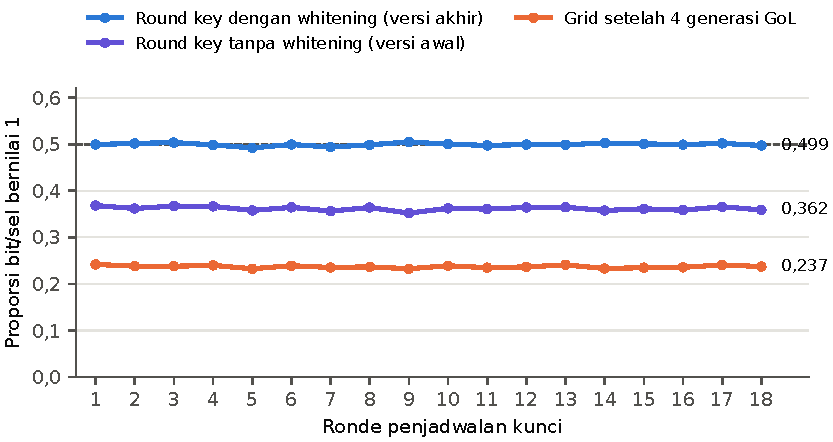
\includegraphics[width=\textwidth]{rk_density.pdf}
    \caption{Proporsi bit 1 pada grid dan \textit{round key} untuk setiap ronde penjadwalan kunci (300 pasangan kunci dan \textit{nonce} acak; angka di kanan = rata-rata 18 ronde; garis putus-putus = 0,5)}
    \label{fig:rk-density}
\end{figure}

Setelah \textit{whitening}, proporsi bit 1 menjadi \textbf{0,499}. Pengujian yang lebih rinci pada 54.000 \textit{round key} (3.000 pasangan kunci dan \textit{nonce} acak) menunjukkan bahwa masih tersisa bias kecil yang bergantung pada posisi bit. Proporsi per posisi berada di rentang 0,471--0,515, dan 3 dari 128 posisi menyimpang secara signifikan dari 0,5 ($|z| > 4$). Bit pada \textit{round key} yang berurutan tidak berkorelasi (koefisien korelasi 0,0001), sehingga bias ini bukan artefak sampel. Penyebabnya kemungkinan struktur spasial pengisian spiral, karena delapan sel yang berasal dari byte materi kunci yang sama saling berkorelasi. Dampaknya sangat kecil: jika setiap posisi dianggap independen, entropi \textit{round key} hanya berkurang sekitar 0,007 bit dari 128 bit. Entropi byte \textit{round key} juga mencapai 7,9981 dari 86.400 byte, sesuai dengan nilai harapan 7,9979 untuk data acak berukuran sama. Uji \code{test\_security} versi akhir juga melaporkan proporsi 0,4985 dan entropi byte 7,9934 (harapan 7,9936 untuk 28.800 byte) (\cref{app:security}).

Kami juga memeriksa apakah langkah paritas menghilangkan informasi kunci. Pada satu pola, setiap byte materi kunci (keluaran SHA-256 yang telah dicampur dengan \textit{nonce}) menentukan 8 bit paritas (satu untuk setiap putaran spiral), tetapi hanya ada 98 kombinasi yang berbeda dari 256 kemungkinan nilai byte (sekitar 6,3 bit informasi). Namun, jika ke-19 pola ($P_0$ dan 18 injeksi ulang dengan \textit{nonce} berbeda) digabungkan, ke-256 nilai setiap byte materi kunci dapat dibedakan pada 50 \textit{nonce} acak yang diuji. Dengan demikian, langkah paritas tidak menyempitkan ruang kunci di tingkat pola.

\subsection{Iterasi Desain Penjadwalan Kunci: Kunci Ekuivalen}
Versi awal melipat kunci yang lebih panjang dari 32 byte dengan XOR, sehingga kunci yang berbeda dapat menghasilkan materi kunci yang sama. Contoh ekstremnya, setiap kunci berbentuk $X \Vert X$ terlipat menjadi 32 byte nol. Pada versi tersebut, \textit{ciphertext} yang dienkripsi dengan kunci \code{"my secret key that is 32 bytes!!"} $\times 2$ dapat didekripsi dengan kunci \code{"A"} $\times 64$.

Versi akhir mengganti pelipatan dengan SHA-256. Karena SHA-256 tahan tabrakan, dua kunci berbeda praktis tidak mungkin menghasilkan materi kunci yang sama, dan setiap bit kunci memengaruhi seluruh 256 bit materi kunci. Pada versi akhir, dekripsi dengan kunci \code{"A"} $\times 64$ gagal dengan \code{ValueError} (\textit{padding} tidak valid), dan \code{test\_security} melaporkan bahwa kedua kunci tidak lagi saling menggantikan. Perlu dicatat bahwa SHA-256 adalah fungsi \textit{hash} yang cepat, bukan KDF untuk kata sandi. Jika kunci berasal dari frasa sandi berentropi rendah, KDF lambat dengan \textit{salt} tetap lebih tepat (\cref{sec:saran}).

\subsection{Integritas dan Malleability}
\label{sec:integritas-keamanan}
Seperti ditunjukkan pada \cref{tab:propagasi}, \algname{} tidak memiliki autentikasi pesan. Penyerang yang mengetahui sebagian isi \textit{plaintext} dapat mengubahnya secara terarah tanpa mengetahui kunci. Pada percobaan dengan mode CBC, membalik bit yang tepat di blok \textit{ciphertext} pertama mengubah \textit{plaintext} blok kedua dari \code{"PAY 0000100 USD\ldots"} menjadi \code{"PAY 9000100 USD\ldots"}, dan dekripsi tetap berhasil tanpa galat. Pada OFB dan CTR, manipulasi ini bahkan lebih mudah karena tidak ada blok yang rusak. Selain itu, fungsi \code{unpad} mengeluarkan dua pesan galat yang berbeda (\code{Invalid padding length} dan \code{Invalid padding sequence}). Jika pesan galat ini terlihat oleh penyerang, ia dapat dimanfaatkan sebagai \textit{padding oracle} pada mode CBC \cite{vaudenay2002}. Kedua masalah ini diatasi dengan skema \textit{Encrypt-then-MAC}, misalnya HMAC-SHA256 atas $N \Vert C$ dengan kunci terpisah \cite{bellare2000, rfc2104}.

\subsection{Kinerja}
Kinerja diukur pada mesin pengembang dengan Python 3.13 (\cref{tab:kinerja}). Penjadwalan kunci hanya dijalankan sekali per pesan, sehingga biaya utamanya adalah 18 ronde Feistel per blok. Laju sekitar 60--70 KB/s membuat implementasi ini cukup untuk berkas berukuran hingga beberapa MB, tetapi berkas 39 MB sudah membutuhkan hampir 10 menit per arah. Kinerja yang rendah ini sebagian besar disebabkan oleh interpretasi Python, bukan oleh rancangan algoritma. Operasi GoL bit-paralel, Kotak-S, dan \code{MixColumns} pada dasarnya hanya terdiri atas operasi bitwise dan \textit{lookup} tabel yang cepat di perangkat keras.

\begin{table}[H]
    \centering
    \caption{Hasil pengukuran kinerja}
    \label{tab:kinerja}
    \begin{tabular}{l r}
        \toprule
        \textbf{Operasi} & \textbf{Waktu / laju} \\
        \midrule
        Penjadwalan kunci (18 \textit{round key}) & 5,7 ms per pesan \\
        Enkripsi satu blok (32 byte) & 474 $\mu$s ($\approx$ 66 KB/s) \\
        Enkripsi / dekripsi \code{image.jpg} (833 KB) & $\approx$ 12 s ($\approx$ 68 KB/s) \\
        Enkripsi / dekripsi \code{video.mp4} (39,2 MB, CBC) & 594 s / 563 s ($\approx$ 64--68 KB/s) \\
        \bottomrule
    \end{tabular}
\end{table}

\section{Ringkasan Hasil Analisis}
\begin{table}[H]
    \centering
    \caption{Ringkasan hasil analisis keamanan}
    \label{tab:ringkasan}
    \small
    \begin{tabularx}{\textwidth}{l Y c}
        \toprule
        \textbf{Aspek} & \textbf{Hasil} & \textbf{Status} \\
        \midrule
        \textit{Round-trip} & teks dan citra pada 5 mode, video pada CBC, 9 panjang \textit{padding} pada 5 mode; \textit{hash} identik & baik \\
        \textit{Avalanche} \textit{plaintext}/kunci & 49,95\% / 50,46\% pada tingkat blok & baik \\
        Difusi & penuh setelah 4 dari 18 ronde & baik \\
        Entropi & sesuai harapan data acak pada semua ukuran & baik \\
        Histogram & rata; kegagalan $\chi^2$ yang sesekali muncul terbukti fluktuasi acak melalui pengujian berulang & baik \\
        Kotak-S & DDT 4/256, LAT 16/256 (setelah iterasi desain) & baik \\
        Batas diferensial terbukti & $\leq 2^{-60}$ (longgar) & perlu kajian \\
        Bit \textit{round key} & proporsi 0,499 setelah \textit{whitening} (sebelumnya 0,362); bias kecil per posisi, kehilangan entropi $\approx$ 0,007 bit & baik \\
        Derivasi kunci & SHA-256, tidak ada lagi kunci ekuivalen $X \Vert X$ & baik \\
        ECB & membocorkan pola di dalam satu pesan & sifat mode \\
        Integritas & tidak ada MAC; \textit{ciphertext} dapat dimanipulasi & lemah \\
        \bottomrule
    \end{tabularx}
\end{table}
